%%%%%%%%%%%%%%%%%%%%%%%%%%%%%%%%%%%%%%%%%%%%%%%%%%%%%%%%%%%%%%%%%%%%%%%%%%%%%%%%
%2345678901234567890123456789012345678901234567890123456789012345678901234567890
%        1         2         3         4         5         6         7         8

\documentclass[letterpaper, 10 pt, conference]{ieeeconf}  % Comment this line out
                                                          % if you need a4paper
%\documentclass[a4paper, 10pt, conference]{ieeeconf}      % Use this line for a4
                                                          % paper

\IEEEoverridecommandlockouts                              % This command is only
                                                          % needed if you want to
                                                          % use the \thanks command
\overrideIEEEmargins
% See the \addtolength command later in the file to balance the column lengths
% on the last page of the document



% The following packages can be found on http:\\www.ctan.org
%\usepackage{graphics} % for pdf, bitmapped graphics files
%\usepackage{epsfig} % for postscript graphics files
%\usepackage{mathptmx} % assumes new font selection scheme installed
%\usepackage{times} % assumes new font selection scheme installed
\usepackage{amsmath} % assumes amsmath package installed
\usepackage{amssymb}  % assumes amsmath package installed
\usepackage{boldline}
\usepackage{array,multirow}
\usepackage{dblfloatfix} 
\usepackage{hyperref}
\usepackage{float}
\usepackage{color}
\usepackage{xfrac}
\usepackage{graphicx}
\graphicspath{ {images/} }
\definecolor{light-gray}{gray}{0.95}
\newcommand{\code}[1]{\colorbox{light-gray}{\texttt{#1}}}
\DeclareMathOperator*{\argmax}{arg\,max}
\DeclareMathOperator*{\maxU}{max}
\usepackage{makecell}
\usepackage{bbm}
\usepackage[table,xcdraw]{xcolor}
\usepackage[flushleft]{threeparttable}
\usepackage[utf8]{inputenc}
\usepackage{capt-of}
\usepackage{mathrsfs}
\usepackage{algorithm}
\usepackage[noend]{algpseudocode}

\title{\LARGE \bf
A Closer Look At The Convergence of Adam and AMSGrad:\\A Reproduction Study
}

\author{ 
	\parbox{2 in}{\centering Tamir Bennatan
         {\tt\small tamir.bennatan@mail.mcgill.ca\\}
         {\tt\small 260614526}}
         \hspace*{ 0.3 in}
         \parbox{2 in}{\centering Lea Collin
         {\tt\small lea.collin@mail.mcgill.ca\\}
         {\tt\small 260618407}}
         \hspace*{0.3 in}
         \parbox{2 in}{\centering Emmanuel Ng Cheng Hin
         {\tt\small emmanuel.ngchenghin@mail.mcgill.ca\\}
         {\tt\small 260615964}}
}



\begin{document}



\maketitle
\thispagestyle{empty}
\pagestyle{empty}

%%%%%%%%%%%%%%%%%%%%%%%%%%%%%%%%%%%%%%%%%%%%%%%%%%%%%%%%%%%%%%%%%%%%%%%%%%%%%%%%
\begin{abstract}
This is filler. Here goes a short abstract. This is filler. Here goes a short abstract. This is filler. Here goes a short abstract. This is filler. Here goes a short abstract. This is filler. Here goes a short abstract. This is filler. Here goes a short abstract. This is filler. Here goes a short abstract. This is filler. Here goes a short abstract. This is filler. Here goes a short abstract. This is filler. Here goes a short abstract. This is filler. Here goes a short abstract. This is filler. Here goes a short abstract. This is filler. Here goes a short abstract. 
\end{abstract}

%%%%%%%%%%%%%%%%%%%%%%%%%%%%%%%%%%%%%%%%%%%%%%%%%%%%%%%%%%%%%%%%%%%%%%%%%%%%%%%%
\section{INTRODUCTION}

Amongst the deep learning community, Stochastic Gradient Descent (SGD) is the predominant method of training deep neural networks. As researchers and practitioners continue to experiment with larger networks with parameter spaces reaching hundreds of millions of dimensions, it has become of increasingly important in recent decades to optimize SGD, so that it may train large networks faster and more effectively. 

One such optimization to SGD is \emph{Adam} (Kingma, Ba; 2015). Inspired by previous variants of SGD which  apply time varying learning rates and momentum terms such as AdaGrad (Duchi et al.,
2011) and RMSProp (Tieleman \& Hinton, 2012), Adam adjusts the learning rates and momentum terms associated with each paramter of a network using an eponential moving averages. In recent years, Adam has been shown to be effective in meany deep learning settings, and is considered a state of the art technique. 

In the paper \emph{On the Convergence of Adam and Beyond}, authors Sashank, Kale and Kumar (2018) present a defect in the Adam method. Since Adam uses exponential moving averages of squared past gradients, the influence on past paramter updates drops off quickly - effectively limiting the reliance of parameter updates to a small set of recent gradients. The authors show that because of this property, Adam will fail to converge in convex optimization problems where large, informative gradients occur infrequently. 

The authors propose a new optimization scheme - \emph{AMSGrad}, which aims to remedy this issue in Adam. To demonstrate that AMSGrad performs better than Adam, they devise a syntethic convex optimization problem, and show that AMSGrad converges to the optimzal solution, while Adam does not. They then train modest neural networks on the widely used MNIST and CIFAR-10 datasets using the Adam and AMSGrad optimizers, and show that AMSGrad converges to a lower loss than Adam. 

In this paper, we recreate the experiments described in the paper\footnote{We refer to \emph{On the Convergence of Adam and Beyond} as simply \emph{``the paper"}, and \emph{``the authors"} as the authors of this paper throughout.} and aim to reproduce the authors' results. We compare our results with those of the authors, and discuss the challenges in recreating the experiments described in this paper. Finally, we present a brief sensitivity analysis, to gauge the variability in our findings.

\section{AMSGrad: LONG TERM MEMORY OF GRADIENTS}

Adaptive optimization procedures such as Adam yield different effecive learning rates for each of the different parameters of a model. Adam computes the effective learning rate using an exponential moving average of past squared gradients. 

If we consider a model with a single parameter, $\theta$, then Adam uses the following update step to optimize the function $f(x)$ at time $t$:

\begin{algorithm}
\caption{Adam Update Rule}\label{Adam-update}
\begin{algorithmic}[1]
\State $g_t = \nabla_{\theta}f_t(x_t)$
\State $m_t = \beta_{1t}m_{t-1} + (1 - \beta_{1t})g_t$ 
\Comment{Adaptive Momentum}
\State $v_t = \beta_2{v_{t-1}} + (1-\beta_2)g_t^2$
\Comment{Adaptive learning rate}
\State $\theta_{t + 1} := \theta_t - \alpha{v_t}$
\end{algorithmic}
\end{algorithm}
Where $\alpha$ is the learning rate, and $(\beta_1, \beta_2)$ are hyperparameters chosen from the range $(0,1)$.

The exponential moving average terms on lines 2 and 3 of Alg. 1 reduce the reliance of each update on past gradients geometrically. The authors show that because of this property, the effective learning rate of each parameter is not guarenteed to be non-decreasing, which causes convergence issues in particular settings. 

To account for this, the authors modify Adam to ``remember" large gradients from further in the past:

\begin{algorithm}
\caption{AMSGrad Update Rule}\label{Adam-update}
\begin{algorithmic}[1]
\State $g_t = \nabla_{\theta}f_t(x_t)$
\State $m_t = \beta_{1t}m_{t-1} + (1 - \beta_{1t})g_t$ 
\State $v_t = \beta_2{v_{t-1}} + (1-\beta_2)g_t^2$
\State $\hat{v_t} = max(\hat{v}_{t-1}, v_t)$
\Comment{Propogate large updates}
\State $\theta_{t + 1} := \theta_t - \alpha{\hat{v_t}}$
\end{algorithmic}
\end{algorithm}

Line 4 of Alg. 2 enables AMSGrad to propogate the large gradients into the future, which increases their affect on future updates. The authors show that after making this small adjustment, AMSGrad guarentees non-increasing effective learning rates, and favorable convergence behaviour.

To illistrate this, the authors propose a simple convex function on the domain $x \in [-1,1]$.:
\[
    f(x) = 
    \begin{cases}
     	Cx, \hspace{5mm} \text{for } t \text{ mod 3 = 1} \\
        -x, \hspace{5mm} \text{otherwise}
    \end{cases}
\]
for $C>2$. The minimum value of  the value of $f$ is achieved at $x=-1$. However, the authors show that Adam converges to the suboptimal solution of $x = 1$, due to the fact that the large gradients with magnitude $C$ are recieved in large intervals. The influence of the large gradient $C$ disappears too quickly to counteract the gradients of $-1$, which moves the algorithm in the wrong direction. AMSGrad, on the other hand, is designed to account for these settings, and minimizes this function without difficulty.

\section{Experiments}


The authors ran several experiments to compare the performance of ADAM and AMSGrad. In this section, we 
describe the experiments run by the authors, and their reported results. 

\subsection{Synthetic Experiments}

The authors construct two convex functions on the domain $x \in [-1,1]$, designed to highlight Adam's shortcomings:

\[
    f_{t}(x) = 
    \begin{cases}
     	1010x, \hspace{5mm} \text{for } t \text{ mod 101 = 1} \\
        -10x, \hspace{5mm} \text{otherwise}
    \end{cases}
\]
where $t$ is the time step at which the function is evaluated, and:

\[
    f(x) = 
    \begin{cases}
     	1010x, \hspace{5mm} \text{with probability 0.01}\\
        -10x, \hspace{5mm} \text{otherwise}
    \end{cases}
\]

Both functions reach a global minimum at $x = -1$. The first is refered to as the ``online setting", and the second as the ``stochastic setting."

In the first experiment, the authors use Adam and AMSGrad to minimize both functions, and compare the convergence behaviour of each optimizer. The authors fix the values of  $\beta_{1}$ and $\beta_{2}$ as the authors at 0.9 and 0.99, respectively, and perform a grid search to find a learning rate $\alpha$ which yields good convergence for both optimizers. 

\subsection{Logistic Regression on MNIST}

The authors then investigated the performance of the algorithm on a logistic regression problem. They used the MNIST dataset, which contains 70,000 28x28 images of handwritten digits, labeled as one of 10 classes. The authors decrease the learning rate over time, where the effective learning rate $\alpha_t$ at time $t$ is defined as $\alpha / \sqrt{t}$. The authors train using minibatches of size of 128, and fix  $\beta_{1}$ as 0.9. They then perform grid search to select a value for $\beta_2$ in the range $(0.99, 0.999)$, based on what value yields the lowest validation loss for each optimizer. 

\subsection{Feedforward Neural Network on MNIST}

The authors trained a feedforward neural network (FFNN) with one hidden layer on the MNIST dataset as well. The hidden layer consists of 100 neurns, and use the ReLU nonlinearity. The authors fix $\beta_{1} = 0.9$, and use a grid to select $\beta_{2}$ from the range $(0.99, 0.999)$, based on which value yields the lowest validation loss for each optimizer.

\subsection{Convolutional Neural Network on CIFAR-10}

Finally, the authors experiment with a larger convolutional neural network (CNN), designed to classify images in the CIFAR-10 dataset. CIFAR-10 consists fo 60,000  32 x 32, labeled as one of 10 classes.

The authors specify the architecture that they used (named \emph{Cifarnet}), which consists of two convolutional layers, max-pooling and batch-normilization layers, and two fully connected layers (see appendix 1 for a detailed specification of the architecture.)

The authors trained CifarNet using a minibath of size 128 using each of the two optimizers.The authors fix $\beta_{1} = 0.9$, and perform a grid search to select $\beta_{2}$ from the range $(0.99, 0.999)$.

\subsection{Results}

The authors present their results by visualizing the losses of their models achieved during training using Adam and AMSGrad for each of the experiments discussed [figure 1]. These plots show that in all of the experiments, models trained using AMSGrad achieved lower losses and converged faster than those trained with Adam. These results bolster the author's claims that AMSGrad's dependence on long term gradients indeed ameliorates its convergence behavior.
\begin{figure*}
\begin{minipage}{1\textwidth}
\centering
\begin{minipage}{0.55\textwidth}
  \centering
  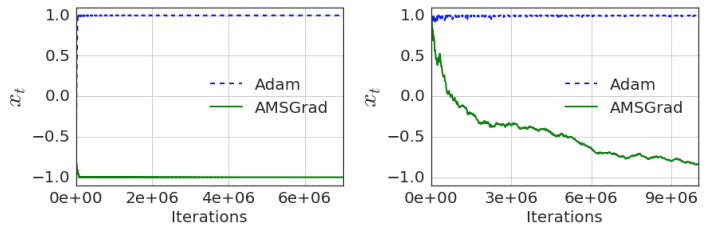
\includegraphics[width=1\linewidth]{OG_synthetic.png}
  \label{fig:test2}
\end{minipage}% 
\centering
\break
\begin{minipage}{0.9\textwidth}
  \centering
  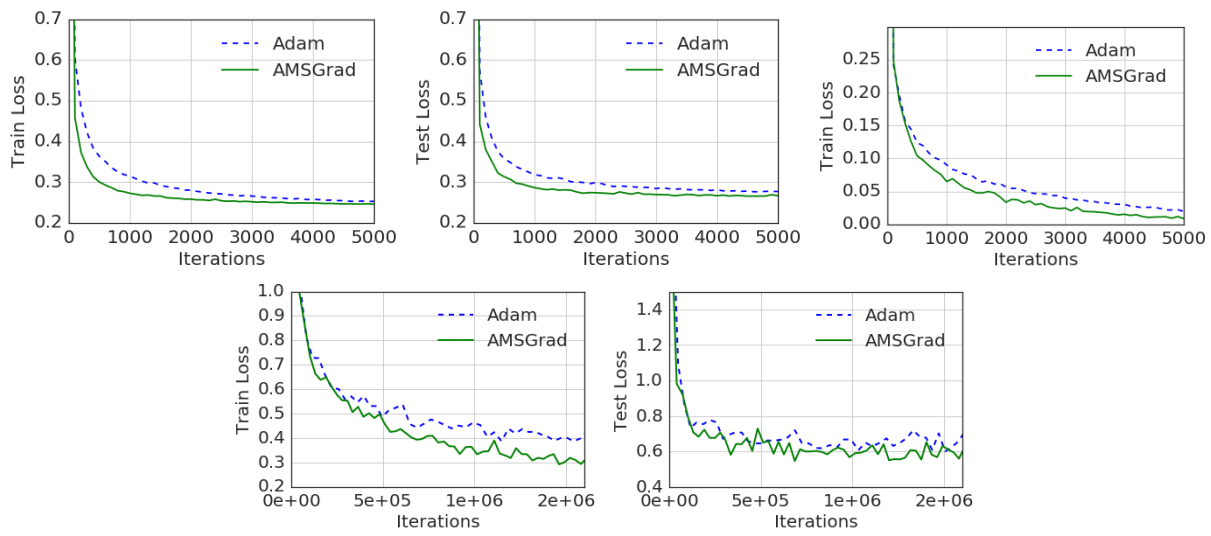
\includegraphics[width=1\linewidth]{OG_results_nets.png}
  \label{fig:test2}
\end{minipage}%
\end{minipage}
\caption[]{Top: location of $x_t$ in the online and stochastic syntetic experiments, respectively. \\
Middle: performance of ADAM and AMSGrad on logistic regression (left and center) 1-hidden layer feedforward neural network (right) on MNIST.\\
Bottom: training and test loss of ADAM and AMSGrad with respect to iterations for CifarNet.\\
These graphs were taken directly from the paper \emph{On the Conergence of Adam and Beyond} (Sashank, Kale, Kumar; 2018).} 
\end{figure*}    
   
    
\section{Hindrances to Reproducability}  

Although the authors take care to justify their claims and experiments with theory, they omit several key details that make it difficult to recreate their experiments exactly. These details can be broadly categorized into those which concern the experimental setup, those which conern the model architectures, and those which concern the exact values of model hyperparameters. 

\subsection{Experimental Setup}

In the paper, the models do not specify for how many epochs they trained each of the described classifiers.

Although the images they provide [figure 1] show the number of \emph{iterations} they trained for, it is difficult to decifer what these iterations represent. 

For the models trained on MNIST, the authors show that they trained for 5,000 iterations. If an iteration is defined as one batch parameter update\footnote{The authors use mini-batches of size 128 in all experiments. Thus, in the $50,000$ training examples of MNIST, one epoch would consist of $50000/128 \approx 390$ batch parameter updates.}, then 5,000 iterations would correspond to 10-20 training epochs, which is reasonable. The authors show, however, that they trained CifarNet for over 2 Million iterations. Using this same definition of an iteration, this would correspond to over $5,000$ training epochs. Given the size of CifarNet, we find it dubious that the authors trained for thousands of epochs\footnote{On an NVIDIA Kepler GK104 GRID GPU, one training epoch takes roughly 90 seconds.}.

To overcome this ambiguity, we determined a number of training epochs for each model that we found reasonable. We aimed to choose a number of training epochs for each number that gives each model ample time to converge, but that can train in a reasonable time frame. Thus, we trained our logistic regression and feedforwarnd neural network models for 50 epochs, and our CifarNet models for 30 epochs. 

\subsection{Model Architectures}

The authors do not specify several key details of their model architectures. Most severely, they do not specify the loss function they used to learn their parameters. 

In a multi-class classification setting (such as MNIST and CIFAR-10 classification), a natural choice for a loss function is categorical cross-entropy. After running our experiments using categorical-crossentropy, however, we noticed that the scale of our models' losses did not match those reported by the authors. For example, when running a feedforward neural network on MNIST, we observed training losses in roughly the range (1, 6), while the authors report losses in the range (.2, .7). 

Based on these observations, we concluded that the authors must have used a loss function other than categorical-crossentropy. As an alternative, we tried using binary-crossentropy (also known as \emph{multiclass log-loss} in the multiclass setting), which is defned for a $k$ class classification problem as:

\[
Loss(\hat{y}_i, y_i) = -\sum_{k = 1}^K \big( y_{i,k}\log(\hat{y}_{i,k}) + (1 - y_{i,k})\log(1 - \hat{y}_{i,k})  \big)
\]

When using this loss function we found that our observed losses aligned more closesly with those reported by the authors in our experiments regarding the MNIST dataset. However, we observed losses much smaller than those reported by the authors when training CifarNet. 

This could be becuase the authors used different loss functions in their experiments regarding MNIST and CIFAR-10. It could also be that the authors used a loss function other than categorical cross-entropy and multiclass log-loss.

As the paper's results focus on the superiority of AMSGrad over Adam, we decided that the magnitude of the losses observed is less important than the relative magnitute between those achieved when training with AMSGrad, and those achieved when training with Adam. Thus, we proceeded with our experiments using the multiclass log-loss, with knowledge that this loss may be different than one one used by the authors.

\subsection{Model Hyperparameters}

Finally, the authors do not full detail on the hyperparameter they chose for each model. 

In the CifarNet CNN model, an important hyperparameter is the stride length to use in each convoltional layer. Given just the kernel size and number of filters, one cannot deduce the stride length used by the authors\footnote{For the layer to be specified fully, either the stride length or zero-padding length should also be specified.}. Unable to resove this abiguity, we proceeded with our experiments using a stride length of one. Any discrepencies between our results and those reported by the author may be partly due to the use of different stride lengths. 

The authors mention that they tune the learning rate $\alpha$ and the hyperparameter $\beta_2$ using a grid search in each of their experiments. However, they do not specify the hyperparamters they ultimately used. 

This forced us to experiment with large parameter spaces when we recreated their grid searches, as we did not have an approximate neighborhood of values which we know work well in the proposed experiments. As training deep networks such as CifarNet is very slow, exhaustive searches are very costly. Thus, omitting the final hyperparameters introduces computational barriers to reproducing the authors' results well. 

\section{METHODOLOGY}

\textbf{Here lies a brief description of what we did - tuning, training multiple runs.}

\subsection{Hyperparemter Tuning}

\textbf{Here lies details on hyperparameter tuning}

\subsection{Reproduced Experiments}

\textbf{Here lies details on experiments ran - number of runs, configs etc}

\section{RESULTS}

\textbf{Here lies details on results (graphs).}

\section{DISCUSSION AND CONCLUSION}

\textbf{Here lies comparison of our results with authors'. Are they the the same for each model? Are they as conclusive? Are the authors ignoring variability in in their models? }



\section{RESULTS}

The results for the synthetic experiments are shown in Figure 3 (haven't put it in yet). \par
The results for the MNIST and CIFAR-10 experiments are in Figure 4. Similar to what is seen in the results provided by the authors, we have that AMSGrad has a slightly lower loss than ADAM for these experiments. We also observe quite a small loss for our CIFAR-10 experiments, about 0.05 for both training and test losses. This is a much smaller loss than what was observed by the authors, who achieved about 0.3 training loss with AMSGrad and about 0.6 test loss with AMSGrad. We do not know what loss the authors used however, which could be the source of the discrepancy. Overall, the general trends we observe in our results coincide with the general trends reported by the authors. 

\begin{figure*}[]
\centering
\begin{minipage}{0.9\textwidth}
  \centering
  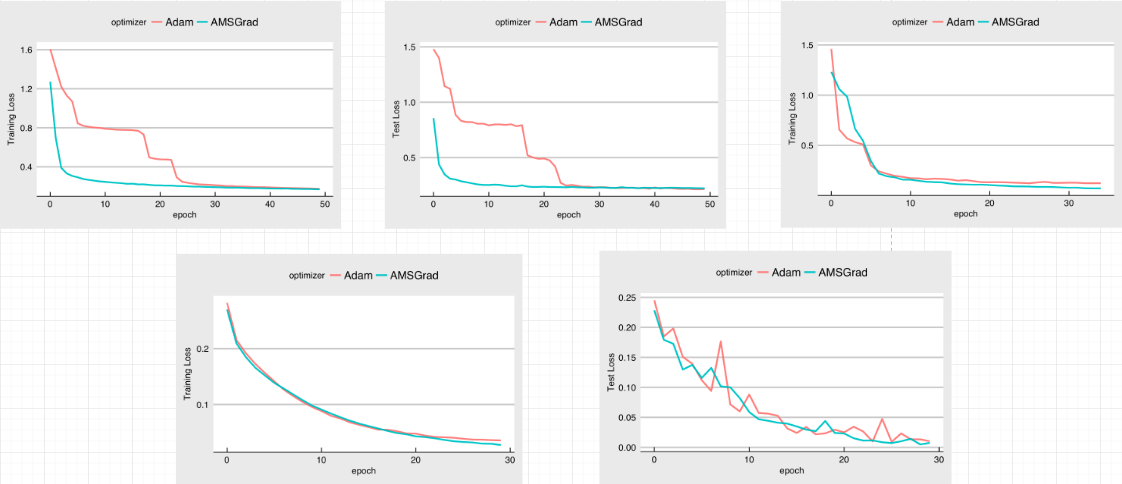
\includegraphics[width=1\linewidth]{Fig4.png}
  \label{fig:test4}
\end{minipage}%
\caption[]{The top row shows performance of ADAM and AMSGrad on logistic regression (left and center) 1-hidden layer feedforward neural network (right) on MNIST. In the bottom row, the two plots compare the training and test loss of ADAM and AMSGrad with respect to iterations for CIFARNET. These graphs are meant to coincide with the graphs in Figure 2, which were graphs provided by the authors.} 
\end{figure*} 

\section{DISCUSSION}
The authors did quite a nice job of describing in detail what they did in each experiment they ran. For example, the full architectures of the two neural networks they trained were fully specified. Additionally, they stated the exact value of hyperparameters they did not tune (for example $\beta_{1}$) and gave a range for $\beta_{2}$ which they did tune. They also mentioned that they used a grid search to tune these parameters, so we knew to do that as well. \par
This is not to say that the authors' work was perfectly reproducible. Though they mentioned the range of $\beta_{2}$ values they tried, they did not give a range of $\alpha$ values for any of the experiments that they ran. Furthermore, though it is likely that they used categorical cross-entropy loss in the classification experiments, they do not explicitly state so. In their results, the authors often plotted the training or test loss against the number of iterations, but they do not define what they consider to be an iteration. We are fairly confident that one iteration means one run through one mini-batch, however, without the authors stating explicitly, we cannot be certain. Because of this, we are unsure of exactly how long the authors ran each experiment. To work around this, we ran each experiment until there was very little change in loss from one epoch to the next, as is usually done and this seems to be what the authors did, since we achieved similar results. However, in terms of absolute reproducibility of their results, this impeded our ability to reproduce the results exactly. \par
The biggest shortcoming of this paper is likely that the authors never state what they got to be the best hyperparameters after performing a grid search. Because we were able to get very similar results to the, we believe that the hyperparameters must be the same, yet we have no way to confirm. \par
Though we were able to produce extremely similar results to those provided in the original paper, these results did not come at a low cost. Because the authors did not provide a range of $\alpha$ values they tried for any of their experiments, we had to use a  wide range in our grid search to ensure that we likely explored all of the same possible values the authors had explored. Grid searches take a long time to run (INSERT LENGTH OF TIME FOR EACH EXPERIMENT HERE). This problem was exacerbated for the CIFAR-10 experiments as CNN's already take a long time to train (about 2 hours) and so to also do a grid search took (about 28 hours?). Thought it was useful that the authors stated they performed a grid search to do all hyperparameter tuning, it would have saved a lot of time and effort if they had simply stated what the best hyperparameters were that they found. This also would have made it much easier to decide if the results were reproducible or not as we would have been able to follow more exactly what the authors did. \par
Furthermore, CNN's also require a GPU to significantly speed up the amount of time required to train. This required us to use Amazon Web Services which required much more setup than simply running all of the code within our own machines. We chose to use Amazon Web Services rather than Google Collab because AWS was something that we had worked with before. Additionally, Google Collab would terminate if we let the screen of the computer turn off and considering we were running the CNNs overnight, this was not ideal. 
\addtolength{\textheight}{-12cm}   % This command serves to balance the column lengths
                                  % on the last page of the document manually. It shortens
                                  % the textheight of the last page by a suitable amount.
                                  % This command does not take effect until the next page
                                  % so it should come on the page before the last. Make
                                  % sure that you do not shorten the textheight too much.

%%%%%%%%%%%%%%%%%%%%%%%%%%%%%%%%%%%%%%%%%%%%%%%%%%%%%%%%%%%%%%%%%%%%%%%%%%%%%%%%



%%%%%%%%%%%%%%%%%%%%%%%%%%%%%%%%%%%%%%%%%%%%%%%%%%%%%%%%%%%%%%%%%%%%%%%%%%%%%%%%
\begin{thebibliography}{99}
\bibitem{c1} R. Sashank, S. Kale, S. Kumar, (2018). On the Convergence of Adam and Beyond. In Proceedings of \emph{International Conference on Learning Representations}, http://https://openreview.net/forum?id=ryQu7f-RZ (link is external)
\bibitem{c2} Diederik P. Kingma and Jimmy Ba (2015). Adam: A method for stochastic optimization. In Proceedings
of \emph{3rd International Conference on Learning Representations, 2015.}
\bibitem{c3} Chollet, Fran\c{c}ois and others, 2015. Keras: \url{https://keras.io}
\bibitem{c4} T. Tieleman and G. Hinton. RmsProp: Divide the gradient by a running average of its recent magnitude.
\bibitem{c5} John C. Duchi, Elad Hazan, and Yoram Singer. Adaptive subgradient methods for online learning
and stochastic optimization. Journal of Machine Learning Research, 12:2121–2159, 2011.

\section*{Blog Posts}

\bibitem{c5} Brownlee, J. (2016, August 9). Tuning optimization parameters using a gridsearch. Retrieved from https://machinelearningmastery.com/grid-search-hyperparameters-deep-learning-models-python-keras/
\bibitem{c6} Korzeniowski, F. (2017, December 22). Experiments with AMSGrad. Retrieved from https://fdlm.github.io/post/amsgrad/

\end{thebibliography}
\newpage
\section{APPENDIX}
\subsection{Appendix 1: Model Architectures}
\begin{figure}[H]
      \centering
      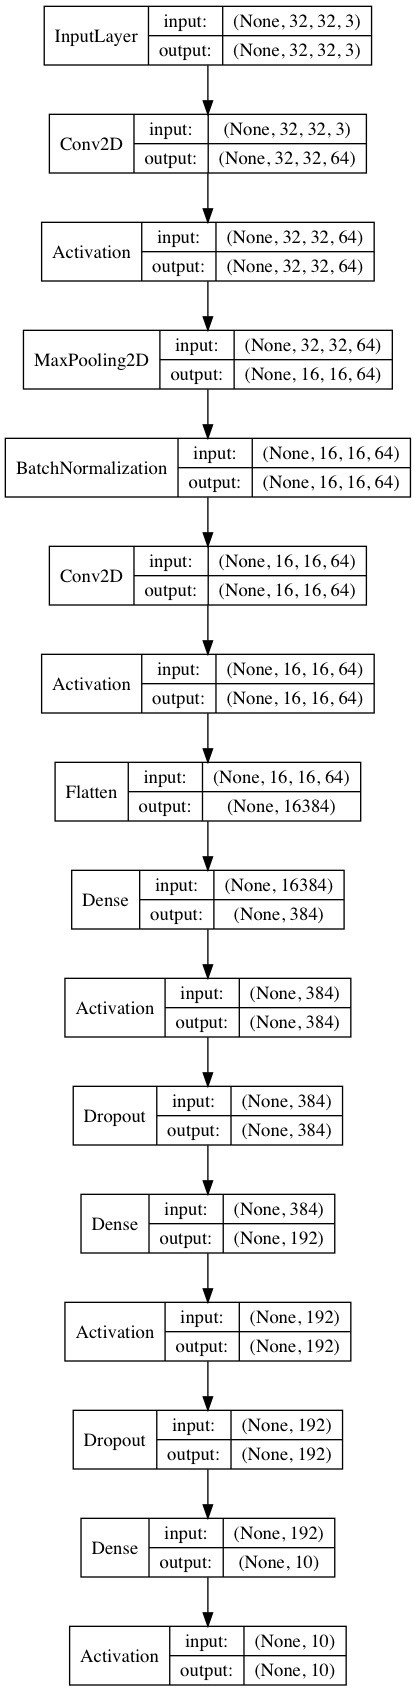
\includegraphics[scale = .3]{cifarnet_model.png}
		\centering
      %\includegraphics[scale=1.0]{figurefile}
      \caption{CifarNet architecture; a deep Convolutional Neural Network designed to classify images in the Cifar-10 dataset.}
      \label{figurelabel}
\end{figure}
    
\begin{figure}[]
      \centering
      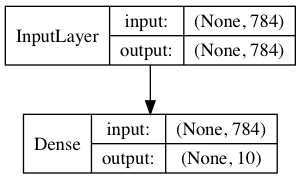
\includegraphics[scale = .3]{logreg_model.png}
		\centering
      \caption{Logistic Regression model, implemented as a feedforward neural network with no hidden layers.}
      \label{figurelabel}
\end{figure}

\begin{figure}[]
      \centering
      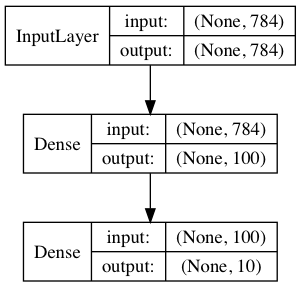
\includegraphics[scale = .3]{ffnn_model.png}
		\centering
      %\includegraphics[scale=1.0]{figurefile}
      \caption{Feedforward Neural Network Architecture, trained on MNIST 28x28 greyscale images.}
      \label{figurelabel}
\end{figure}

%%%%%%%%%%%%%%%%%%%%%%%%%%%%%%%%%%%%%%%%%%%%%%%%%%%%%%%%%%%%%%%%%%%%%%%%%%%%%%%%



\end{document}

